% Onpersoonlijk:
\section{Wat zijn de belangrijke aspecten van de kavels VI en VII?} \label{Wat zijn de belangrijke aspecten van de Kavels VI en VII?}

\subsection{Obstakels}
Er zijn veel aspecten van de kavels VI en VII waar rekening mee moet worden gehouden. Ten eerste is de locatie van de kavels van belang. De kavels maken onderdeel uit van het windenergiegebied Hollandse Kust west en liggen op ongeveer 53 km van de west kust van Nederland en hebben een oppervlakte van circa 176 km\textsuperscript{2}.\cite{SiteDescriptionRVO} De twee kavels zullen elk een offshore windcapaciteit van 700MW realiseren.\cite{SiteDescriptionRVO}\cite{Functies&gebruikHKW}

Om het windpark te ontwerpen dat instaat is dit te bieden zijn verschillende andere gegevens van de kavels belangrijk. Er moet bepaald worden wat de beste positionering is voor de windturbines. Bij de beslissing hiervan moeten aspecten in acht genomen worden, zoals al bestaande en geplande infrastructuur van pijpleidingen en kabels. Daarnaast moet rekening worden gehouden met potentiële magnetische abnormaliteiten zoals genoteerd staat in Appendix C van de locatie beschrijving (zie figuur \ref{fig:obstakels}).\cite{SiteDescriptionRVO}\cite{AppendixC} Uit voorzorg zullen, de windturbines op een minimale afstand van 100 meter van betreffende obstakels geplaatst worden.
\begin{figure}[h]
\centering
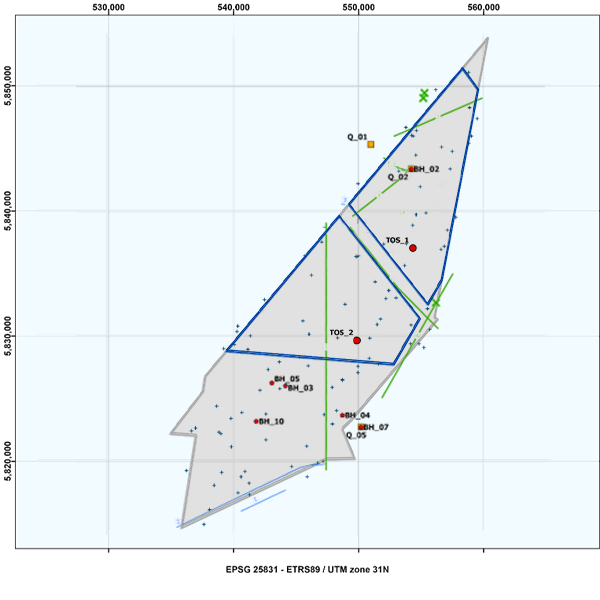
\includegraphics[width=0.5\textwidth]{IMG/data/overzicht/Map_obstakels.png} 
\caption{Map van te vermijden obstakels.}
\label{fig:obstakels}
\end{figure}

\subsection{Wind gegevens}
Er is ook informatie over de kavels die significant is voor het besluit van de windturbines en de oriëntatie hiervan. De informatie die hiervoor belangrijk is, is de winddata, zoals windsnelheden en -richtingen over langere periodes. De gebruikte data bevat de gemeten windsnelheden en -richtingen op de locatie HKW over de afgelopen twee decennia (31-10-1999 tot 31-10-2019) met meetintervallen van 1 uur.\cite{WindData} \cite{WindResourceAssessment} 
Deze metingen zijn gedaan op een hoogte van 100 meter boven het gemiddelde zeeniveau en zijn dus representatief voor de te verwachten winden die de windturbines zullen ervaren. 

Door deze gegevens te analyseren, kan het gemiddelde voor zowel de windsnelheid als de windrichting berekend worden. Echter niet alle gemeten waardes voldoen aan de voorwaarden om mee door te kunnen rekenen. Om te identificeren welke waardes voldoen word de gemiddelde windrichting gehanteerd met een marge ter in acht neming van de invalshoek van de wind en de rotatie mogelijkheden van de turbine. Dit marge is 45$^{\circ}$ in beide richtingen van de gemiddelde windrichting (197,7$^{\circ}$). De windrichtingen die dus voldoen vallen tussen de 152,7$^{\circ}$ en 242,7$^{\circ}$. Uiteraard zullen de turbines tegen de overheersende windrichting in geplaatst worden om de opbrengst te optimaliseren.

Van de gefilterde gegevens is vervolgens gekeken naar de windsnelheden variërend van 0 tot 31 kilometer per uur en is geanalyseerd hoe vaak elke windsnelheid voor komt. De resultaten van deze analyse zijn als volgt:

\[
\begin{tabular}{|c|c|}
\hline
Windsnelheid (m/s) & Aantal keer voorkomend \\
\hline
0 & 108 \\
1 & 555 \\
2 & 1105 \\
3 & 1701 \\
4 & 2169 \\
5 & 2652 \\
6 & 3159 \\
7 & 3610 \\
8 & 3945 \\
9 & 4403 \\
10 & 4589 \\
11 & 4564 \\
12 & 4369 \\
13 & 4026 \\
14 & 3834 \\
15 & 3277 \\
16 & 2923 \\
17 & 2461 \\
18 & 1982 \\
19 & 1551 \\
20 & 1162 \\
21 & 814 \\
22 & 517 \\
23 & 332 \\
24 & 173 \\
25 & 99 \\
26 & 57 \\
27 & 33 \\
28 & 21 \\
29 & 7 \\
30 & 5 \\
31 & 2 \\
\hline
\end{tabular}
\]

De gemiddelde windsnelheid van de ongefilterde data komt uit op 9,74 m/s. Na filtratie is de gemiddelde windsnelheid gelijk aan 11,16 m/s. Dit is een aanzienlijk verschil en toont de significantie van de uitgevoerde filtratie.

Na volledige filtratie van de data blijkt 34,3\% van de gegevens te voldoen. Dit komt overeen met 60206 metingen. Hiermee doorrekenen zal dus accuraat blijven en is daarom ook gedaan. Met de gefilterde 

Daarna is het percentage waarmee elke windsnelheid voorkomt berekend, met behulp van de volgende formule:

\[
\text{Percentage\textsubscript{frequentie}} = \frac{\text{Aantal keren voorkomend bij een bepaalde windsnelheid}}{\text{Aantal keren voorkomend bij alle windsnelheden}}
\]

De volgende stap is berekenen hoeveel dagen elke windsnelheid in een jaar voorkomt en dit omzetten naar uren per jaar met de formule \(365 \times 24 \times \text{Percentage\textsubscript{frequentie}}\). Deze gegevens kunnen dan gebruikt worden om de energieopbrengst van de turbines voor elke windsnelheid te berekenen, waarmee weer verder gerekend kan worden.


\begin{equation} \label{eq:7}
\text{Frequentie windsnelheid in uren/jaar: } 365\times 24\times \text{Percentage\textsubscript{frequentie}}
\end{equation}
\myequations{Berekening: Frequentie windsnelheid}


De verdeling van de frequentie van de windsnelheden over de span van de gemeten periode\cite{WindData} staat in (figuur \ref{fig:Windfrequentie}).
\begin{figure}[H]
\centering
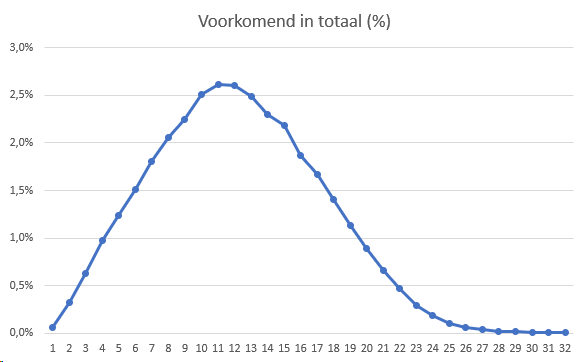
\includegraphics[width=0.7\textwidth]{IMG/data/overzicht/Windfrequentie.png}
\caption{Gegevens: frequentie wind snelheid per jaar.}
\label{fig:Windfrequentie}
\end{figure}

% Er is naar een veelvoud windturbines gezocht en gekeken. Bekeken modellen waren onder andere de volgende:
% \begin{itemize}
%     \item De SG 14-236 DD, 14 MW windturbine van Siemens Gamesa.\cite{SiemensGamesa14MW}
%     \item De V236-15.0, 15 MW windturbine van Vestas.
%     \item De Haliade-X, 12 MW windturbine van GE renewable energy.\cite{GEHalideX}
%     \item 
% \end{itemize}
